% !TeX program = pdflatex
% Documento auxiliar para compilar las tablas de malla.
% Uso: latexmk malla-curricular-tablas-standalone.tex
\documentclass[11pt,a4paper]{article}
\usepackage[margin=1.5cm]{geometry}
\usepackage[utf8]{inputenc}
\usepackage[T1]{fontenc}
\usepackage[spanish,es-tabla]{babel}
\usepackage{lmodern}
\usepackage{array}
\usepackage[table]{xcolor}
\usepackage{colortbl}
\usepackage{booktabs}
\usepackage{multirow}
\usepackage{rotating}
\usepackage{float}
\usepackage{rotfloat}

\definecolor{Celeste-UCR}{RGB}{0,192,243}
\definecolor{Azul-UCR}{RGB}{0,93,164}
\definecolor{Verde-UCR}{RGB}{109,192,103}
\definecolor{Amarillo-UCR}{RGB}{255,224,106}

\title{\textcolor{Azul-UCR}{Malla curricular — tablas resumen}}
\author{}
\date{}

\begin{document}
\maketitle
% =============================================================================
% Tablas de malla curricular.
% Fuente: Documentos/210401-3 Pura.xlsx y 210401-3 Aplicada.xlsx
% Regenerar: python scripts/generate_malla_from_210401.py
% =============================================================================

En este capítulo se presenta la estructura curricular del plan de estudios propuesto así como el análisis realizado para la selección y organización de contenidos. Como parte del proceso de reestructuración de la carrera Bachillerato y Licenciatura en Matemática, se ha considerado la participación del personal docente del departamento que expresó la necesidad de abandonar el modelo actual para pasar a uno más moderno, acorde con las necesidades y demandas del país, con diferentes áreas de especialización.

\section{Malla curricular obligatoria propuesta}

Se presenta, en forma tabular, la estructura curricular propuesta. El detalle de los contenidos de los cursos se encuentra en el siguiente capítulo.

% Estilo compartido para tablas de malla curricular (paleta UCR).
% Requiere: xcolor[table], array, colortbl, rotating, float, hyperref.

\providecolor{Celeste-UCR}{RGB}{0,192,243}
\providecolor{Azul-UCR}{RGB}{0,93,164}
\providecolor{Verde-UCR}{RGB}{109,192,103}
\providecolor{Amarillo-UCR}{RGB}{255,224,106}

\newcommand{\MallaSubsection}[1]{%
  \subsubsection*{\textcolor{Azul-UCR}{#1}}%
}

\newcommand{\MallaSidewayBegin}{%
  \begingroup
  \small
  \setlength{\tabcolsep}{4.5pt}%
  \renewcommand{\arraystretch}{1.2}%
  \arrayrulecolor{Azul-UCR!80}%
  \setlength{\arrayrulewidth}{0.5pt}%
  \begin{sidewaystable}[H]%
  \centering
}

\newcommand{\MallaSidewayEnd}{%
  \end{sidewaystable}%
  \endgroup
}

\newcommand{\MallaTabularBegin}{%
  \rowcolors{3}{white}{Celeste-UCR!12}%
  \begin{tabular}{@{}%
    |c|l|>{\raggedright\arraybackslash}p{5.2cm}|%
    c|c|c|c|c|%
    >{\raggedright\scriptsize\arraybackslash}p{3.9cm}|%
    >{\raggedright\scriptsize\arraybackslash}p{3.3cm}|@{}}
}

\newcommand{\MallaHeader}{%
  \rowcolor{Azul-UCR}%
  \color{white}\bfseries
  Ciclo & Curso & Nombre del curso &
  \multicolumn{4}{c|}{\cellcolor{Azul-UCR}Horas} & Cred. &
  \shortstack{Requisitos y\\ Req. Equivalentes} &
  \shortstack{Correquisitos y\\ Correq. Equivalentes} \\ \hline
  \rowcolor{Celeste-UCR!35}%
  \color{black}\bfseries
  & & & T & P & L & TP & & & \\ \hline
}

\newcommand{\MallaCicloTotal}[2]{%
  \rowcolor{Verde-UCR!28}%
  \multicolumn{10}{|l|}{\textit{Créditos ciclo #1: #2}} \\ \hline
}

\newcommand{\MallaTotalFinal}[2]{%
  \rowcolor{Amarillo-UCR!45}%
  \multicolumn{10}{|r|}{\textbf{#1: #2}} \\ \hline
}

% Sigla clicable hacia el programa (\hypertarget del cuerpo).
% Uso: \MallaSigla{MA0151}  o  \MallaSigla[destino]{MA0615}
\makeatletter
\newcommand{\MallaSigla}[2][]{%
  \def\MallaSigla@opt{#1}%
  \ifx\MallaSigla@opt\empty
    \hyperlink{#2}{#2}%
  \else
    \hyperlink{#1}{#2}%
  \fi
}
\makeatother


\MallaSidewayBegin
\MallaSubsection{Bloque común (ciclos I a III)}

\MallaTabularBegin
\MallaHeader
1 & EF- & ACTIVIDAD DEPORTIVA &  &  &  &  & 0 &  &  \\
1 & EG-I & CURSO INTEGRADO DE HUMANIDADES I &  &  &  &  & 6 &  &  \\
1 & \MallaSigla{MA0151} & FUNDAMENTOS DE ÁLGEBRA, TRIGONOMETRÍA Y GEOMETRÍA ANALÍTICA &  &  &  &  & 3 &  &  \\
1 & \MallaSigla{MA0152} & MATEMÁTICA EXPLORATORIA &  &  &  &  & 3 &  &  \\
1 & RP- & REPERTORIO &  &  &  &  & 3 &  &  \\
\MallaCicloTotal{1}{15}
2 & EG- & CURSO DE ARTE &  &  &  &  & 2 &  &  \\
2 & EG-II & CURSO INTEGRADO DE HUMANIDADES II &  &  &  &  & 6 & EG-I &  \\
2 & LM-3039 & INGLÉS PARA ESTADÍSTICA I &  &  &  & 4 & 3 & XS-1130 o MA-0152 &  \\
2 & \MallaSigla{MA0251} & INTRODUCCIÓN AL CÁLCULO EN UNA VARIABLE &  &  &  &  & 3 & MA0151 Fundamentos de Álgebra, Trigonometría y Geometría Analítica & MA0252 Introducción a las Demostraciones \\
2 & \MallaSigla{MA0252} & INTRODUCCIÓN A LAS DEMOSTRACIONES &  &  &  &  & 4 & MA-0152 Matemática Exploratoria &  \\
\MallaCicloTotal{2}{18}
\end{tabular}

\vspace{1cm}

\MallaTabularBegin
\MallaHeader
3 & SR-I & SEMINARIO DE REALIDAD NACIONAL I &  &  &  &  & 2 & EG-II &  \\
3 & \MallaSigla{MA0361} & ALGEBRA LINEAL I &  &  &  &  & 3 & MA0252 Introducción a las Demostraciones &  \\
3 & LM-3040 & INGLÉS PARA ESTADÍSTICA II &  &  &  & 4 & 3 & LM-3039 &  \\
3 & \MallaSigla{MA0351} & INTRODUCCIÓN AL CÁLCULO EN VARIAS VARIABLES &  &  &  &  & 3 & MA-0251 Cálculo en una variable & MA-0361 Algebra Lineal I \\
3 & \MallaSigla{MA0341} & MATEMÁTICA COMPUTACIONAL & 4 &  &  &  & 3 & MA0251 Cálculo en Una Variable & MA0361 Álgebra Lineal I \\
\MallaCicloTotal{3}{17}
\MallaTotalFinal{Total créditos bloque común}{50}
\end{tabular}
\MallaSidewayEnd

\MallaSidewayBegin
\MallaSubsection{Énfasis en matemática pura (ciclos IV a VIII)}

\MallaTabularBegin
\MallaHeader
4 & SR-II & SEMINARIO DE REALIDAD NACIONAL II &  &  &  &  & 2 & SR-I &  \\
4 & \MallaSigla{MA0461} & ALGEBRA LINEAL II &  &  &  &  & 3 & MA0361 Álgebra Lineal I &  \\
4 & \MallaSigla{MA0451} & PRINCIPIOS DE ANÁLISIS EN UNA VARIABLE &  &  &  &  & 4 & MA-0351 Cálculo en Varias Variables & MA0461 Álgebra Lineal II \\
4 & \MallaSigla{MA0471} & INTRODUCCIÓN A LA GEOMETRÍA DIFERENCIAL &  &  &  &  & 3 & MA-0351 Cálculo en Varias Variables &  \\
4 & \MallaSigla{MA0496} & TEORÍA DE NÚMEROS &  &  &  &  & 3 & MA-0252 Introducción a las Demostraciones &  \\
\MallaCicloTotal{4}{16}
\end{tabular}
\MallaSidewayEnd

\MallaSidewayBegin
\MallaTabularBegin
\MallaHeader
5 & \MallaSigla{MA0561} & ALGEBRA ABSTRACTA I &  &  &  &  & 4 & MA-0461 Algebra Lineal II y MA-0496 Teoría de Números &  \\
5 & \MallaSigla{MA0551} & PRINCIPIOS DE ANÁLISIS EN VARIAS VARIABLES &  &  &  &  & 4 & MA-0451 Principios de Análisis I y MA-0461 Álgebra Lineal II &  \\
5 & \MallaSigla{MA0515} & ECUACIONES DIFERENCIALES &  &  &  &  & 4 & MA-0451 Principios de Análisis I y MA-0461 Álgebra Lineal II &  \\
5 & OPT- & OPTATIVA DE OTRA DISCIPLINA &  &  &  &  & 3 &  &  \\
\MallaCicloTotal{5}{15}

\MallaHeader
6 & \MallaSigla{MA0661} & ALGEBRA ABSTRACTA II &  &  &  &  & 5 & MA-0561 Algebra Abstracta I &  \\
6 & \MallaSigla{MA0635} & INTRODUCCIÓN A LA TOPOLOGÍA &  &  &  &  & 4 & MA-0551 Principios de Análisis II &  \\
6 & \MallaSigla{MA0641} & ANÁLISIS NUMÉRICO I & 5 &  &  &  & 4 & MA-0341 Matemática Computacional y MA-0515 Ecuaciones Diferenciales Ordinarias &  \\
6 & OPT- & OPTATIVA DE OTRA DISCIPLINA &  &  &  &  & 3 &  &  \\
\MallaCicloTotal{6}{16}
\end{tabular}
\MallaSidewayEnd

\MallaSidewayBegin
\MallaTabularBegin
\MallaHeader
7 & \MallaSigla{MA0705} & ANÁLISIS REAL I &  &  &  &  & 5 & MA-0635 Topología General &  \\
7 & \MallaSigla{MA0702} & ANÁLISIS COMPLEJO &  &  &  &  & 4 & MA-0635 Topología General &  \\
7 & \MallaSigla{MA0780} & COMUNICACIÓN EN LAS CIENCIAS & 2 &  &  & 4 & 2 & Haber aprobado al menos uno de: MA-0661 Algebra Abstracta II, MA-0635 Introducción a la Topología MA-0647 Modelación Matemática o MA-0641 Análisis Numérico I &  \\
7 & OPT-001 & Optativa núcleo en matemática pura &  &  &  &  & 4 &  &  \\
\MallaCicloTotal{7}{15}

\MallaHeader
8 & \MallaSigla[MA0781Pura]{MA0781} & PRÁCTICA PROFESIONAL EN MATEMÁTICA PURA &  & ¿? &  & ¿? & 6 & Haber aprobado al menos uno de: MA-0661 Algebra Abstracta II o MA-0635 Topología General &  \\
8 & OPT-001 & Optativa núcleo en matemática pura &  &  &  &  & 8 &  &  \\
8 & OPT-003 & Optativa general en matemática &  &  &  &  & 4 &  &  \\
\MallaCicloTotal{8}{18}
\MallaTotalFinal{Total créditos bachillerato pura}{130}
\end{tabular}
\MallaSidewayEnd

\MallaSidewayBegin
\MallaSubsection{Énfasis en matemática aplicada (ciclos IV a VIII)}

\MallaTabularBegin
\MallaHeader
4 & \MallaSigla{MA0461} & ALGEBRA LINEAL II &  &  &  &  & 3 & MA0361 Álgebra Lineal I &  \\
4 & \MallaSigla{MA0451} & PRINCIPIOS DE ANÁLISIS EN UNA VARIABLE &  &  &  &  & 4 & MA-0351 Cálculo en Varias Variables & MA0461 Álgebra Lineal II \\
4 & \MallaSigla{CA0721} & PROBABILIDAD & 5 &  &  &  & 4 & (CA-0351, CA-0352) o MA-0351 &  \\
4 & \MallaSigla[CA0203]{CA-0204} & HERRAMIENTAS DE CIENCIA DE DATOS I &  &  &  & 5 & 4 & (CA-0101, CI-0112) o MA-0341 &  \\
\MallaCicloTotal{4}{16}
\end{tabular}
\MallaSidewayEnd

\MallaSidewayBegin
\MallaTabularBegin
\MallaHeader
5 & SR-II & SEMINARIO DE REALIDAD NACIONAL II &  &  &  &  & 2 & SR-I &  \\
5 & \MallaSigla{MA0551} & PRINCIPIOS DE ANÁLISIS EN VARIAS VARIABLES &  &  &  &  & 4 & MA-0451 Principios de Análisis I y MA-0461 Álgebra Lineal II &  \\
5 & \MallaSigla{MA0515} & ECUACIONES DIFERENCIALES &  &  &  &  & 4 & MA-0451 Principios de Análisis I y MA-0461 Álgebra Lineal II &  \\
5 & \MallaSigla{CA0303} & ESTADÍSTICA ACTUARIAL I &  &  &  & 5 & 4 & MA-0720 o CA-0721, CA-0204 &  \\
5 & OPT- & OPTATIVA DE OTRA DISCIPLINA &  &  &  &  & 3 &  &  \\
\MallaCicloTotal{5}{17}

\MallaHeader
6 & \MallaSigla{MA0641} & ANÁLISIS NUMÉRICO I & 5 &  &  &  & 4 & MA-0341 Matemática Computacional y MA-0515 Ecuaciones Diferenciales Ordinarias &  \\
6 & \MallaSigla{MA0635} & INTRODUCCIÓN A LA TOPOLOGÍA &  &  &  &  & 4 & MA-0551 Principios de Análisis II &  \\
6 & \MallaSigla{MA0647} & Modelación matemática & 5 &  &  &  & 4 & MA-0515 &  \\
6 & OPT- & Optativa de otra disciplina &  &  &  &  & 3 &  &  \\
\MallaCicloTotal{6}{15}
\end{tabular}
\MallaSidewayEnd

\MallaSidewayBegin
\MallaTabularBegin
\MallaHeader
7 & \MallaSigla{MA0705} & ANÁLISIS REAL I &  &  &  &  & 5 & MA-0635 Topología General &  \\
7 & \MallaSigla{MA0702} & ANÁLISIS COMPLEJO &  &  &  &  & 4 & MA-0635 Topología General &  \\
7 & \MallaSigla[CA0411AnalisisDatos]{CA-0411} & ANÁLISIS DE DATOS I &  &  &  & 5 & 4 & CA-0307 &  \\
7 & \MallaSigla{MA0780} & COMUNICACIÓN EN LAS CIENCIAS & 2 &  &  & 4 & 2 & Haber aprobado al menos uno de: MA-0661 Algebra Abstracta II, MA-0635 Introducción a la Topología MA-0647 Modelación Matemática o MA-0641 Análisis Numérico I &  \\
\MallaCicloTotal{7}{15}

\MallaHeader
8 & \MallaSigla[MA0781Aplicada]{MA0781} & PRÁCTICA PROFESIONAL EN MATEMÁTICA APLICADA &  & ¿? &  & ¿? & 6 & Haber aprobado al menos uno de: MA-0647 Modelación Matemática, MA-0641 Análisis Numérico I o MA-0635 Topología General &  \\
8 & OPT-002 & Optativa núcleo en matemática aplicada &  &  &  &  & 8 &  &  \\
8 & OPT-003 & Optativa general en matemática &  &  &  &  & 4 &  &  \\
\MallaCicloTotal{8}{18}
\MallaTotalFinal{Total créditos bachillerato aplicada}{131}
\end{tabular}
\MallaSidewayEnd

\MallaSidewayBegin
\MallaSubsection{Énfasis en matemática pura (licenciatura, ciclos IX y X)}

\MallaTabularBegin
\MallaHeader
9 & \MallaSigla[MA0781SEDPura]{MA0781} & SEMINARIO DE ESTUDIOS DIRIGIDOS EN MATEMÁTICA PURA I & 2 &  &  & 19 & 7 & MA-0781 Práctica profesional en matemática pura &  \\
10 & OPT-001 & Optativa núcleo en matemática pura &  &  &  &  & 4 &  &  \\
9 & OPT-003 & Optativa general en matemática &  &  &  &  & 4 &  &  \\
\MallaCicloTotal{9}{15}
10 & \MallaSigla[MA0881Pura]{MA0881} & SEMINARIO DE ESTUDIOS DIRIGIDOS EN MATEMÁTICA PURA II & 2 &  &  & 19 & 7 & MA-0781 Seminario de estudios dirigidos en matemática pura I &  \\
10 & OPT-003 & Optativa general en matemática &  &  &  &  & 8 &  &  \\
\MallaCicloTotal{10}{15}
\MallaTotalFinal{Total créditos licenciatura pura}{30}
\end{tabular}
\MallaSidewayEnd

\MallaSidewayBegin
\MallaSubsection{Énfasis en matemática aplicada (licenciatura, ciclos IX y X)}

\MallaTabularBegin
\MallaHeader
9 & \MallaSigla[MA0781SEDAplicada]{MA0781} & SEMINARIO DE ESTUDIOS DIRIGIDOS EN MATEMÁTICA APLICADA I & 2 &  &  & 19 & 7 & MA-0781 Práctica profesional en matemática aplicada &  \\
9 & OPT-002 & Optativa núcleo en matemática aplicada &  &  &  &  & 4 &  &  \\
9 & OPT-003 & Optativa general en matemática &  &  &  &  & 4 &  &  \\
\MallaCicloTotal{9}{15}
10 & \MallaSigla[MA0881Aplicada]{MA0881} & SEMINARIO DE ESTUDIOS DIRIGIDOS EN MATEMÁTICA APLICADA II & 2 &  &  & 19 & 7 & MA-0781 Seminario de estudios dirigidos en matemática aplicada I &  \\
10 & OPT-003 & Optativa general en matemática &  &  &  &  & 8 &  &  \\
\MallaCicloTotal{10}{15}
\MallaTotalFinal{Total créditos licenciatura aplicada}{30}
\end{tabular}
\MallaSidewayEnd

\begin{figure}
\centering
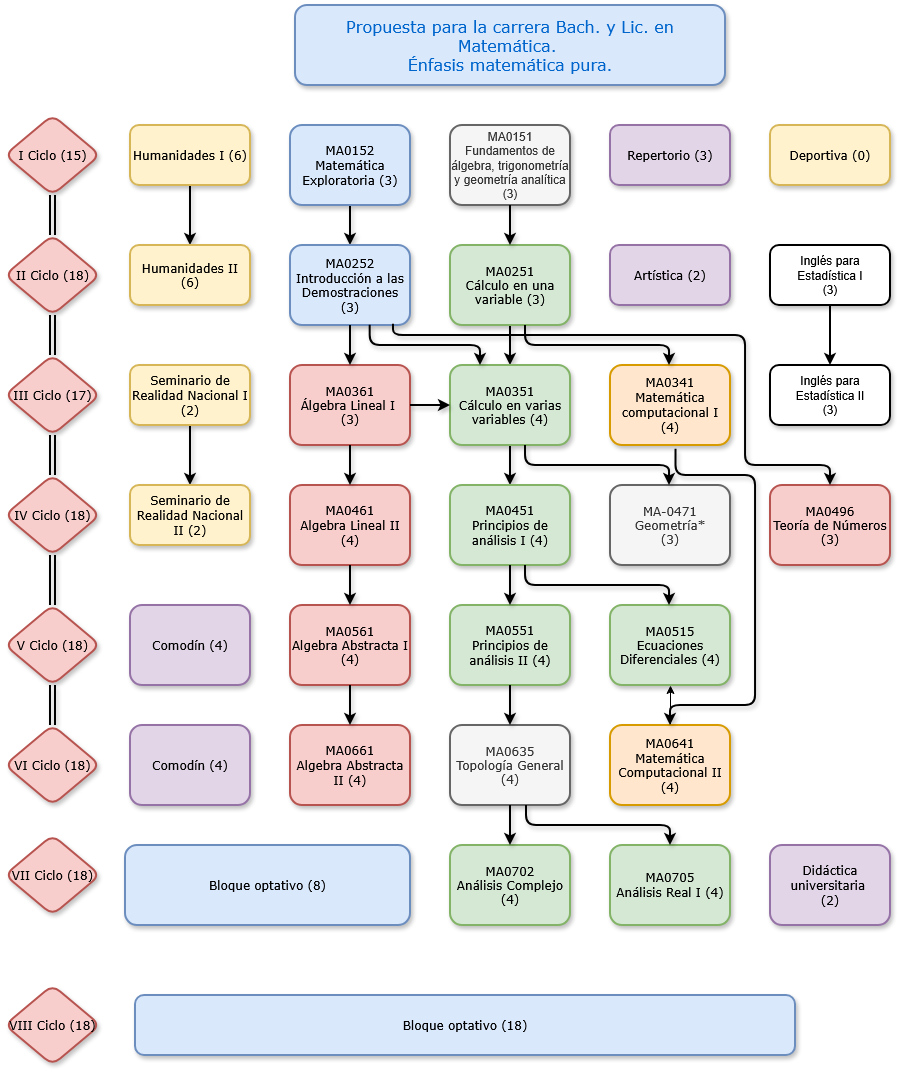
\includegraphics[width=0.75\textwidth]{propuesta_pura}
\caption{Diagrama de plan de Bachillerato y Licenciatura en Matemática con énfasis en Matemática Pura}
\end{figure}

\begin{figure}
\centering
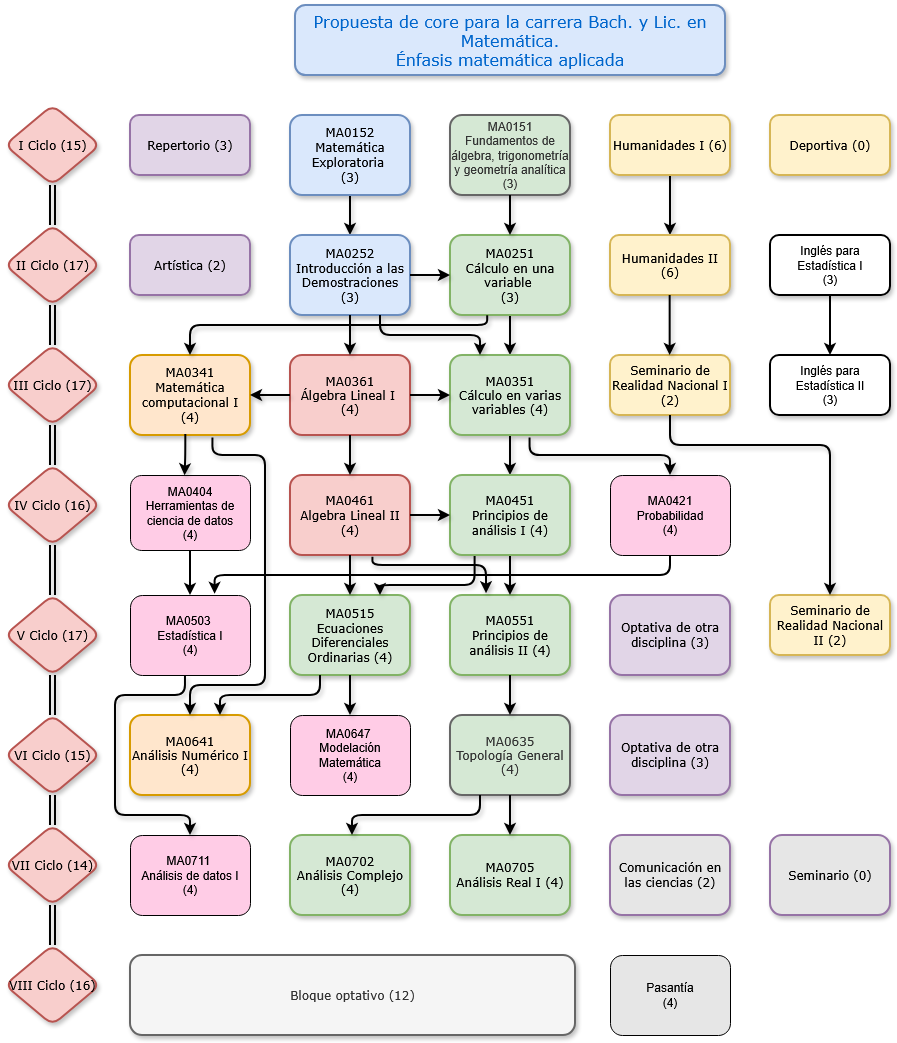
\includegraphics[width=0.75\textwidth]{propuesta_aplicada}
\caption{Diagrama de plan de Bachillerato y Licenciatura en Matemática con énfasis en Matemática Aplicada}
\end{figure}

\subsection{Requisitos de graduación}

\subsubsection{Bachillerato en matemática, ambos énfasis}

Se requiere de la asistencia, a lo largo de la carrera, a diez (10) actividades académicas válidas , por ejemplo:
\begin{enumerate}
    \item Charlas del Coloquio del Departamento de Matemáticas.
    \item Seminarios, conferencias o ciclos especiales anunciados por el departamento como válidos para este curso.
    \item Otras actividades académicas que la Dirección del Departamento disponga expresamente, con indicaciones oportunas.
\end{enumerate}

\subsubsection{Licenciatura en matemática, ambos énfasis}

Se requiere de la asistencia, a lo largo de la carrera, a cinco (5) actividades académicas válidas, distintas a las empleadas para cumplir el requerimiento similar de bachillerato, por ejemplo:
\begin{enumerate}
    \item Charlas del Coloquio del Departamento de Matemáticas.
    \item Seminarios, conferencias o ciclos especiales anunciados por el departamento como válidos para este curso.
    \item Otras actividades académicas que la Dirección del Departamento disponga expresamente, con indicaciones oportunas.
\end{enumerate}
\end{document}
